\documentclass[A4paper,oneside,fleqn,11pt]{article}

% This first part of the file is called the PREAMBLE. It includes
% customizations and command definitions. The preamble is everything
% between \documentclass and \begin{document}.

%Cambiamos un poquito los márgenes%
\addtolength{\oddsidemargin}{-1in}
\addtolength{\evensidemargin}{-1in}
\addtolength{\textwidth}{2in}
\addtolength{\topmargin}{-1in}
\addtolength{\textheight}{2in}

\usepackage{mathtools}
\usepackage{graphicx}              % to include figures
\usepackage{amsmath}               % great math stuff
\usepackage{amsmath,scalerel}
\usepackage{amsfonts}              % for blackboard bold, etc
\usepackage{amsthm}                % better theorem environments
\usepackage{amssymb}
\usepackage{mathrsfs}
\usepackage[spanish]{babel}
\usepackage[utf8]{inputenc}
\usepackage{hyperref}
\usepackage{multicol}
\usepackage{tikz-cd}
\usepackage{amsmath}
\usepackage[linesnumbered,ruled]{algorithm2e}
\usepackage{algpseudocode}
\usetikzlibrary{calc}
\usetikzlibrary{matrix}
\usepackage{graphicx,wrapfig,lipsum}

\graphicspath{ {Grphs/} }


\setcounter{tocdepth}{3}% to get subsubsections in toc

\let\oldtocsection=\tocsection

\let\oldtocsubsection=\tocsubsection

\let\oldtocsubsubsection=\tocsubsubsection

% various theorems, numbered by section

\newtheorem{teo}{Teorema}[section]
\newtheorem{lem}[teo]{Lema}
\newtheorem{prop}[teo]{Proposición}
\newtheorem{cor}[teo]{Corolario}
\newtheorem{crit}[teo]{Criterio}
\newtheorem{propi}[teo]{Propiedad}

\theoremstyle{definition}
\newtheorem{ejcio}[teo]{Ejercicio}
\newtheorem{conj}[teo]{Conjetura}
\newtheorem{obs}[teo]{Observación}
\newtheorem{defn}[teo]{Definición}
\newtheorem{ax}[teo]{Axioma}
\newtheorem{ex}[teo]{Ejemplo}

\newcommand{\bd}[1]{\mathbf{#1}}  % for bolding symbols
\newcommand{\cl}[1]{\overline{#1}} 
\newcommand{\CC}{\mathbb{C}}
\newcommand{\RR}{\mathbb{R}}      % for Real numbers
\newcommand{\ZZ}{\mathbb{Z}}      % for Integers
\newcommand{\NN}{\mathbb{N}}
\newcommand{\QQ}{\mathbb{Q}}
\newcommand{\FF}{\mathbb{F}}
\newcommand{\col}[1]{\left[\begin{matrix} #1 \end{matrix} \right]}
\newcommand{\comb}[2]{\binom{#1^2 + #2^2}{#1+#2}}
\newcommand{\eps}{\varepsilon}
\renewcommand{\hom}{\mathrm{Hom}}
\let\oldemptyset\emptyset
\let\emptyset\varnothing
\DeclareMathOperator{\id}{id}
\DeclareMathOperator{\mcm}{mcm}
\DeclareMathOperator{\mcd}{mcd}
\DeclareMathOperator{\ord}{ord}
\DeclareMathOperator{\im}{im}
\DeclareMathOperator{\End}{End}
\DeclareMathOperator{\Aut}{Aut}
\DeclareMathOperator{\sg}{sg}
\DeclareMathOperator{\cok}{cok}
\DeclareMathOperator{\ext}{Ext}
\DeclareMathOperator{\Obj}{Obj}
\DeclareMathOperator{\rank}{rk}
\DeclareMathOperator{\gr}{gr}
\DeclareMathOperator{\car}{char}
\DeclareMathOperator{\Nil}{Nil}
\DeclareMathOperator{\spec}{Spec}
\DeclareMathOperator{\ev}{ev}
\DeclareMathOperator{\ann}{Ann}
\DeclareMathOperator{\tr}{Tr}
\DeclareMathOperator*{\bigcdot}{\scalerel*{\cdot}{\bigodot}}
\def\acts{\curvearrowright}
\def\stca{\curvearrowleft}

\setcounter{tocdepth}{10}
\setcounter{secnumdepth}{10}

\usepackage[utf8]{inputenc}
\usepackage{fancyhdr}

 \chead{Algo III, TP2, Chehebar, Duran, Somacal}
 
\title{Algoritmos y Estructuras de Datos III, TP2}
\author{Nicolás Chehebar, Matías Duran, Lucas Somacal}
\date{}


\begin{document}

\pagenumbering{roman}
\pagenumbering{arabic}
\maketitle
\tableofcontents
\clearpage

\section{Problema 1}
\subsection{El Problema}

\subsubsection{Descripcion}
Planteado de otra forma, el problema a resolver consiste en una situación en la que tenemos $n$ trabajos $t_{1},t_{2},...,t_{n}$ y dada cualquier división de los trabajos en dos secuencias $A=(t_{a_{1}},t_{a_{2}},..., t_{a_{|A|}})$ y $B=(t_{b_{1}}, t_{b_{2}},...,t_{b_{|B|}})$  con $a_{i}<a_{j} \land b_{i}<b_{j} si i<j$ (cada secuencia representa los trabajos que realizo una máquina) tiene asociado un costo; donde este viene dado por la suma del costo de $A$ y el de $B$. El costo de $A$ es  $\sum_{i=1}^{|A|} costo (t_{a_{i}},t_{a_{i-1}})$  donde $costo$ es una función que toma valores en $\NN_{0}$ y $costo(t_{i},t_{j})$ esta definidio si $i>j$ con $i \in [1,2,..,n] \land j \in [0,1,..,n-1]$ y represnta el costo de poner el trabajo i sobre el j (el costo de poner sobre el trabajo $t_{0}$ es el de ponerlo sobre la máquina vacía y $a_{0}=0$). El costo de $B$ se calcula análogamente. 

El problema pide dados los trabajos y la funcion de costo, dar $A$ o $B$ que minimice el costo y decir cuanto es este costo (basta dar uno de los dos ya que el otro se deduce por ser el complemento -en el conjunto de trabajos-)
\subsubsection{Ejemplos}
\begin{itemize}
\item En el caso en que la entrada es $\begin{matrix}
  4 &  &  &  \\
  2 &  &  &  \\
  300 & 3 &  &  \\
  300 & 3 & 3 &  \\
  300 & 3 & 3 & 3 
\end{matrix}$ tenemos 4 trabajos que sacando el primero son excesivamente caros de poner por primera vez en una maquina, luego si ponemos todos en la misma, el costo sera $2+3+3+3=11$ y una máquina tendrá todos los trabajos (si todos no estan en la misma, en algun momento pagamos $300$ y el costo ya seria mayor a $11$).
\item En el caso en que la entrada es $\begin{matrix}
  4 &  &  &  \\
  2 &  &  &  \\
  4 & 1 &  &  \\
  300 & 3 & 300 &  \\
  300 & 300 & 300 & 3 
\end{matrix}$ tenemos 4 trabajos, ponemos el primero en una maquina y nos da costo $2$, si bien en el proximo paso lo mejor es poner el nuevo trabajo encima (si hicieramos un algoritmo goloso), en ese caso el siguiente trabajo costara $300$ haciendo el total $>299$, y si no hibieramos puesto el segundo encima, si bien costaba mas en ese paso, reducía el costo del próximo, dando un costo total de $12$ estando los trabajos 1, 3 y 4 en una maquina.
\end{itemize}


\subsection{El Algoritmo}

\subsubsection{La función de dinámica}
Para resolver el problema, utilizaremos programación dinámica. La idea de esto se basa en que la solución de nuestro problema es calculable en base a la solucion de subproblemas (utilizamos optimalidad de subproblemas). Definimos así $f(q,h)$ como la función que asigna el mínimo costo posible para llegar al trabajo $q$-ésimo hecho (habiendo hecho de la 1 hasta la q inclusive) con el trabajo $h$ como el último que se hizo en algunas de las máquinas. Tomamos como dominio de la $f$ a los $q \in [1,2,...,t] \land h \in [0,1,...,q-1]$. donde $h=0$ significa que hay una maquina vacía. Es clave notar que siempre que luego de que realizamos el trabajo $q$ en una de las máquinas estará en el tope dicho trabajo, por ende basta definir que hay en la otra. Definimos a continuación la función para los valores en el dominio ya mencionado:

\begin{equation}
    f(q,h) =
    \begin{cases*}
       costo(q,0) & $si$  $q=1$  $\land$  $h=0 $\\
       f(q-1,h)+costo(q,q-1) & $si  h < q-1 $\\
       \displaystyle \min_{0 \leq h \leq q-2} {f(q-1,h)+precios[q][h]}       & caso contrario (h=q-1)
    \end{cases*}
  \end{equation}

Esta función hace efectivamente lo que queremos:
\begin{itemize}

 \item En el primer caso lo hace pues si $q=1$ esto implica $h=0$ por restricciones de dominio y es la minima cantidad dado que coloqué solo el primer trabajo, pues si o si el costo será el de colocar la primera sobre la maquina vacía, por ende será el mínimo.
 \item En el segundo caso también lo hace pues si esta un trabajo $h<q-1$ en una máquina es porque el ultimo trabajo colocado (el q) se colocó en la otra, por ende previo a finalizar el trabajo $q$, estaba en una máquina el $q-1$ y en otra el $h$. Más aún sabemos que el q lo colocamos sobre el $q-1$. Supongamos $f(q,h)$ el costo mínimo dado el trabajo $q$ hecho y el trabajo $h$ en alguna impresora (analogo para $f(q-1,h)$), si es $f(q,h)<f(q-1,h)+costo(q,q-1)$ luego es absurdo pues $f(q-1,h)$ no es el minimo, ya que hago la secuencia que da el mínimo en $q$ trabajos hechos con $h$ en una máquina sin el ultimo paso (resto su costo, o sea el de poner a $q$ sobre $q-1$) y me queda que tengo una forma de tener $q-1$ trabajos hechos con $h$ en una maquina con costo $f(q,h)-costo(q,q-1)<f(q-1,h)$ lo que es absurdo pues $f(q-1,h)$ era el minimo.
 \item En el tercer caso también sucede pues si está el trabajo $q-1$ en una máquina con la impresión $q$ ya hecha, es porque la impresión $q$ se colocó sobre alguna impresión $h$ con $0 \leq h \leq q-2$. Dada dicho trabajo, de forma totalmente análoga al caso de arriba, debe ser el mínimo buscado con $q$ trabajos hechos y el $q-1$ en una máquina $f(q,q-1)= f(q-1,h)+costo(q,h)$. Luego como no se cual trabajo de todos pudo haber sido, me quedo con el mínimo moviendo los h en el rango dado.
  \end{itemize}
Así, definimos una función que resuelve el problema pedido si hayamos el $\displaystyle \min_{0 \leq h \leq t-1} {f(t,h)}  $ pues es el mínimo costo de realizar hasta el trabajo $t$ (o sea todos) con el trabajo $h$ en alguna máquina (me fijo todos los escenarios posibles como puede terminar la otra máquina, o sea todos los posibles $h$). 

Así, podemos implementar la $f$ dada, donde podemos ir recordando los valores que toma $f$ y evitar calcularlos varias veces. Más aún podríamos mantener una lista (ordenada) de cuales son los elementos que hay en alguna máquina y cada vez que agregamos un trabajo, checkeamos si lo agregamos sobre el ultimo de la lista y en ese caso lo incluimos al final de esta (sino es porque fue a la otra máquina).

Lo que sucede es que tenemos varios subproblemas y en este caso siempre resolvemos todos, por lo que no parece tener una clara ventaja hacerlo top-down. Más aún, hacerlo bottom-up nos permitirá solo guardarnos los subproblemas relativos a tener hecho exactamente hasta el anterior trabajo (con $q-1$ y para todos los $h$, los menores no los utilizo en el calculo de $f(q,h)$), o sea nos reduce la complejidad espacial! Ya que incialmente debíamos guardar el valor de $f$ para todo $q \in [1,2,...,t] \land h \in [0,1,...,q-1]$ lo que era $\mathcal{O}(n^2)$, y de esta forma solamente guardamos los valores para $q-1$ lo que es $\mathcal{O}(n)$.

 Veamos todo esto en un pseudocódigo:
\subsubsection{El Pseudocódigo}

Cabe aclarar que en el pseudcódigo (como también en la implementación) numeramos los trabajos desde 0 a exceión de en $costos$ (que es una matriz) en el segundo indice, los trabajos estan numerados desde 1 (ya que el 0 se reserva para el costo de poner sobre la máquina vacía).

\begin{algorithm}[H]
    \SetKwInOut{Input}{Input}
    \SetKwInOut{Output}{Output}

    \underline{Dinámica} $(trabajos,costo)$\;
    \Input{$trabajos \in \NN_{0}$; $costo \in \NN_{0}^{trabajos \times trabajos}$}
    \Output{$costo \in \NN_{0}$,$lista$ vector enteros}
    
    Inicializo en $0$ $actualcosto$ y $anteriorcosto$ vectores de enteros (de tamaño $trabajos$);
    
    Inicializo en vectores vacíos $actuallista$ y $anteriorlista$ vectores de vectores de enteros (de tamaño $trabajos$);
    
    \For{q $\in [0,1,..,trabajos)$}{
    	\For{h $\in [0,1,..,q)$}{
    	
    		$actualcosto[h]=anteriorcosto[h]+costo[q][q]$;
    		
    		$actuallista[h]=anteriorlista[h]$;
    		
    		\If{Estaba $q-1$ en $anteriorlista[h]$}
        	{
        		Agrego $q$ a $anteriorlista[h]$; 
        	}
        	
    		$actualcosto[q]=min(actualcosto[q],anteriorcosto[h]+costos[q][h])$;
    		
    		Recuerdo en $elegido$ el $h$ que consiguió el minimo;
   		 }
   		 
    $actuallista[q]=anteriorlista[elegido]$;
    
    \If{NO Estaba $q-1$ en $anteriorlista[elegido]$}
        	{
        		Agrego $q$ a $anteriorlista[elegido]$; 
        	}
    anteriorcosto=actualcosto;
    
	anteriorlista=actuallista;
    }
    
     $ costo$ = minimo de $actualcosto$ (se alcanza en $actualcosto[posicion]$);
     
     $lista = actuallista[posicion]$;
     
      return $costo$, $lista$;    
      
      \caption{Devuelve el mínimo costo de entre todas las formas posibles de realizar todas las impresiones}   
\end{algorithm}

En el pseudocódigo basicamente lo que hacemos es aplicar la $f$ pero en orden, es importante esto ya que hay que tener cuidado en el orden en que resolvemos las dependencias (es porque estamos haciendo bottom-up). Es claro que cada fila, usa la fila anterior, o sea para calcular $f(q,h)$ para todo $h$ uso todos los valores de $f(q-1,h)$ para todo $h$. Por esto es que ambos for se anidan de dicha manera. Al principio del for actualizamos el costo segun nos dice la $f$ y la lista de los trabajos que hay en alguna máquina se modifica solo si era el de la máquina que tenía a $q-1$ ya que es a la que le agrego el trabajo $q$. Además, como voy a recorrer todos los $h$, voy actualizando el $actualcosto[q]$ si tengo un menor $anteriorcosto[h]+costos[q][h]$; una vez que iteré en todos los h calculé el minimo que es $f(q,q-1)$. Ahí salimos del primer for y como hacía con $actuallista[h]$ actualizo si corresponde la $actuallista[q]$. Finalmente, antes de pasar a la siguiente iteración pongo en $anteriorcosto$ el $actualcosto$ y en $ anteriorlista$ la $actuallista$, ya que en la proxima iteración los actuales serán anteriores y sobre actual pisaré y guardaré nuevos resultados. Finalmente, se devuelve el mínimo buscado y su lista asociada ( lo que nos pedían era $\displaystyle \min_{0 \leq h \leq t-1} {f(t,h)}  $ que en nuestro caso es el minimo de $actualcosto$.



\subsection{Complejidad}

Cabe aclarar que para el análisis de complejidad tomaremos $n$ como la cantidad de trabajos. Como pudimos ver en la explicación de la función de dinámica, tenemos $n^2$ subproblemas y cada uno se resuelve en  $\mathcal{O}(1)$ salvo los subproblemas donde$ h=q-1$ que toman $\mathcal{O}(n)$. Luego tengo $\mathcal{O}(n^2)$ subproblemas (son $n^2$ en total y le saco los que no se resuelven en $\mathcal{O}(1)$ que son $n$)  resueltos en $\mathcal{O}(1)$ cada uno y $\mathcal{O}(n)$ subproblemas (hay uno por cada $q$) resueltos en $\mathcal{O}(n)$ cada uno. Luego se deduce que la complejidad sera $\mathcal{O}(n*n)+\mathcal{O}(n^2 *1)=\mathcal{O}(n^2)$

Más aún esto se ratifica si miramos el pseudocódigo ya que realizamos todas operaciones que son $\mathcal{O}(n)$ u $\mathcal{O}(n)$ fuera del ciclo (inicialización o recorrido de vectores de tamaño a lo sumo $n$). Veamos que sucede dentro del ciclo: tenemos dos ciclos anidados que se ejecuta cada uno  a lo sumo $n$ veces, por ende todo se ejecuta a lo sumo $n^2$ veces y todo lo de adentro son operaciones $\mathcal{O}(1)$ (checkear si $q-1$ esta en $anteriorlista[h]$ es $\mathcal{O}(1)$ porque inserto siempre ordenado y si es un elemento, es el ultimo; lo mismo vale para checkear si $q-1$ esta en $anteriorlista[elegido]$).Luego salimos del segundo for (el anidado)y cabe aclarar que copiar el vector $actualcosto$ y $actuallista$ no es $\mathcal{O}(1)$ sino $\mathcal{O}(n)$, pero esta solo en uno de los ciclos, por lo que se repite $n$ veces y aporta una complejidad de $n* \mathcal{O}(n)= \mathcal{O}(n^2)$. Por ende en el ciclo tenemos $n^2 *\mathcal{O}(1)+ \mathcal{O}(n^2) = \mathcal{O}(n^2)$ y sumado a lo que esta fuera del ciclo nos da $\mathcal{O}(n)+ \mathcal{O}(n^2) = \mathcal{O}(n^2)$

\subsection{Experimentación}


\subsubsection{Contexto}
La experimentacion se realizó toda en la misma computadora, cuyo procesador era Intel(R) Atom(TM) CPU N2600 @ 1.60GHz, de 36 bits physical, 48 bits virtual, con una memoria RAM de 2048 MB.  Para experimentar, se calculó el tiempo que tardaba el algoritmo sin considerar el tiempo de lectura y escritura ni el tiempo que llevaba armar la matriz (ya que se leía un dato, se escribía la matriz y luego se leia el siguiente). 
El tiempo se medía no como tiempo global sino como tiempo de proceso, calculando la cantidad de ticks del reloj (con el tipo clock\_t de C++) y luego se dividìa el delta de ticks sobre CLOCKS\_PER\_SEC. En todos los experimentos el tiempo se mide en segundos. 
\subsubsection{Experimentos}

\begin{wrapfigure}{R}{0.4\textwidth}
\centering
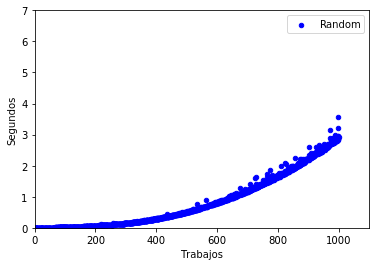
\includegraphics[width=0.4\textwidth]{r.png}
\caption{ Gráfico de segundos de ejecución en función de cantidad de trabajos para instancias aleatorias.}
\end{wrapfigure}
Para empezar a experimentar, se corrió el programa con una serie de $2000$ casos generados aleatoriamente donde aleatoriamente fue con una cantidad de trabajos aleatoria entre $1$ y $10^3$  con una distribución uniforme 
\footnote{ se utilizó la función rand() de librerías de C++ en el rango correspondiente, para mas detalle ver http://en.cppreference.com/w/cpp/numeric/random/rand }
en dicho intervalo. Para la matriz de costos, también se tomo para cada celda un costo aleatorio generado de la misma forma con un costo entre $1$ y $10^6$. A continuación graficamos estas instancias:



Como podemos ver en la Figura 1, pareciera haber un gráfico semejante a una parábola lo que ratificaría la relación cuadrática que propusimos entre la cantidad de trabajos y la cantidad de operaciones realizadas. Sin embargo no nos da del todo información para aseverar eso este gráfico,ya que podría tratarse de alguna función con crecimiento similar. Es por esto que se realizó un gráfico de la relación entre tiempo de ejecución y $trabajos^2$ y si la relación es efectivamente cuadrática este gráfico debería ser constante. Como se puede ver en el gráfico de la figura 2 efectivamente se trata de una constante, lo que verifica nuestra hipótesis y complejidad teórica de la relación cuadrática de dependencia entre la cantidad de operaciones y de trabajos. Podemos observar que no pareciera haber practicamente dispersión, ni mejores ni peores casos, analizaremos esto luego.

\break

\begin{wrapfigure}{l}{0.25\textwidth}
\centering
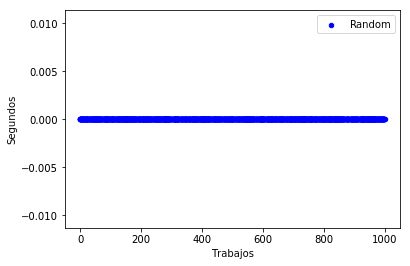
\includegraphics[width=0.25\textwidth]{Escuad.png}
\caption{ Gráfico de segundos de ejecución en función de cantidad de trabajos al cuadrado para instancias aleatorias.}
\end{wrapfigure}

Primero, debemos notar que segun el análisis realizado, en el tiempo de ejecución solo influye la cantidad de trabajos, más alla del costo que pueda tener cada trabajo ya que en lo unico que influye es en la suma (y como trabajamos con enteros acotados, no influye considerablemente en el tiempo de ejecución la suma). Por esto se ejecutaron las mismas $2000$ instancias que se ejecutaron sumando una constante $k$ que se movio entre $10^i$ con $i=1,2,3,4,5,6,7,8,9$ a todo costo y no cambió considerablemente el tiempo de ejecución (notar que no cambia el resultado de cuales trabajos quedan en una máquina respecto de la ejecución respecto de no haber sumado la constante) en todos los $i$ como vemos a continuación en los casos $i=4$ e $i=8$ en las figuras 3, 4 y 5

\vspace{5mm}

\begin{figure}[h!]
  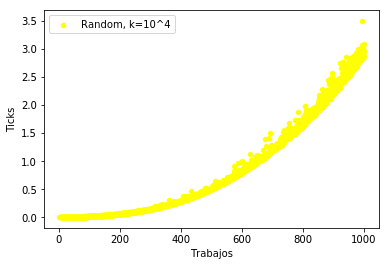
\includegraphics[scale=0.4]{r4.png}
  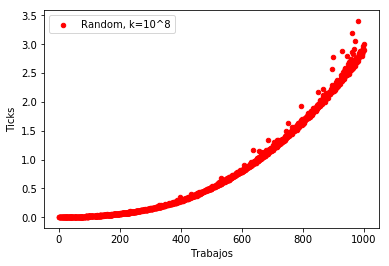
\includegraphics[scale=0.4]{r8.png}
  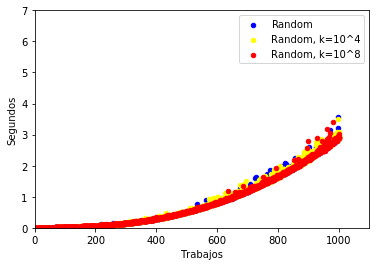
\includegraphics[scale=0.4]{r48.png}
  
\end{figure}
\scriptsize{Figura 3: Gráfico de segundos de ejecución en función de cantidad de trabajos par instancias generadas aleatoriamente, sumando $k=10^4$ en costos}

\scriptsize{Figura 4: Figura 3: Gráfico de segundos de ejecución en función de cantidad de trabajos par instancias generadas aleatoriamente, sumando $k=10^8$ en costos}

\scriptsize{Figura 5: Figura 3: Gráfico de segundos de ejecución en función de cantidad de trabajos par instancias generadas aleatoriamente (en azul), sumando $k=10^4$ (amarillo) y sumando $k=10^8$ (rojo) en costos}
\normalsize

Podemos ver que en todos los casos la dependencia sigue siendo, en rasgos generales la misma, cuadrática (se verifico haciendo el gráfico de $segundos / trabajos^2$ para cada i, los excluimos por una cuestión de espacio, pero todos resultaron constantes). Más aún al comparar instancias de diversos $i$ podemos ver que tienen similar tiempo de ejecución lo que nos indica que (sumado a que tomamos costos aleatorios) no hay influencia de los costos en el tiempo de ejecución, lo que tiene sentido por lo que hace el algoritmo y la complejidad teorica calculada


Como decidimos implementar el algortimo de forma Bottom-Up siempre calculamos todos los subproblemas, esto es una ventaja en el sentido de que siempre todas las instancias de igual cantidad de trabajos tardan lo mismo, como se vio a lo largo de esta experimentacion, por lo que no hay mejores ni peores casos. Al ver la implementación y el pseudocódigo podemos ver que lo que realizamos depende exclusivamente de la cantidad de trabajos total (los costos solo cambian el resultado de cada cuenta, pero no la cantidad de operaciones ni su orden). También tomar esta decisión de implementar Bottom-Up nos permitió ahorrar en memoria ya que no requeríamos memorizar todos los subproblemas, sino que solo utilizabamos la información del subproblema anterior. La única desventaja es que a veces respecto de Top-Down, se calculan todos los subproblemas y no solo los necesarios. Pero si nos detenemos a ver la f que definimos al explicar el algoritmo (como ya también explicamos antes) siempre se van a calcular todos los subprobemas pues son todos necesarios, por ende esa tampoco es una ventaja del Top-Down en este caso. Todo esto se pudo ver experimentalmente ya que todas las instancias tuvieron un tiempo de ejecución muy similar y la dispersión fue practicamente nula.

\subsection{Conclusiones}

Concluimos entonces que la complejidad es de $\mathcal{O}(n^2)$ como se vio teóricamente y además se pudo verificar de forma experimental. Como se analizó al implementar bottom-up se resolvían todos los subproblemas siempre, por lo que (lo que también se vió experimentalmente) no había diferencia entre casos, no había ni peores ni mejores casos, todas las instancias de igual cantidad de trabajos tomaban, practicamente, el mismo tiempo de ejecución. Más aún se vió también experimentalmente que (como se esperaba y se deducía del algoritmo) no había influencia alguna de los valores de los costos en el tiempo de ejecución.

\section{Problema 2}
\subsection{El Problema}

\subsubsection{Descripcion}
Si nos abstraemos de los detalles del problema, este nos describe una situación en la cual tenemos un grafo $G$ (no orientado) conexo con pesos no negativos. Lo que nos piden en la parte 1 del problema es encontrar un conjunto de aristas $E' \subseteq X(G)$ del grafo que cumpla que la suma de sus costos sea la mínima posible (minimizar $\sum_{e \in E'} {peso(e)}$ y que el subgrafo $H$ con nodos $V(G)$ y aristas $E'$ sea conexo. En la parte dos
del problema nos piden, dado un $E'$ que cumple lo antes descripto, elegir un nodo $v \in V(G)$ tal que si consideramos el subgrafo $H$ sin pesos, minimice la máxima distancia de $v$ a otro nodo (minimice $\max_{w\in V(H)}{distancia(v,w)}$).

\subsubsection{Ejemplos}
\begin{itemize}

\item Si consideramos $K_{n}$  (el grafo completo de n vertices) con pesos constantes, todos 1 por ejemplo, la solución será cualquier conjunto de aristas que conecte todos los vertices (son al menos $n-1$ aristas) y con exactamente $n-1$ aristas se alcanza el minimo (pues cada arista es de peso positivo, si no tuviese la minima cantidad de aristas saco una y disminute el peso). Así, la solución tendra peso $(n-1)*1=n-1$ y podemos elegir tales aristas que cumplan que el subgrafo sea conexo (tomo la arista $(i,i+1)$ con $i=1,2,...,n-1$ donde los nodos estan numerados $1,...,n$). Esta sería entonces una solución posible
\item Si consideramos $C_{n}$ (el ciclo simple de n vertices) con pesos todos distintos positivos, la solución debe tener la minima cantidad de aristas posibles (pues cada arista es de peso positivo, si no tuviese la minima cantidad de aristas saco una y disminute el peso) y para que sea conexo estas son $n-1$. Luego basta excluir solo una arista y como quiero minimizar el peso y saque cual saque queda conexo, saco la de mayor peso y ya (es unica la solución en este caso, pues son todos distintos y la  arista de peso maximo es única). Las aristas buscadas serán todas menos la excluida y el peso, la suma de sus pesos.

\end{itemize}


\subsection{Consultora 1}

\subsubsection{El algoritmo}
Si nos detenemos a evaluar lo que pide la primer parte del problema, notamos que la solución debe permitir que sea conexo el grafo (debe tener $n-1$ aristas al menos) y debe minimizar la cantidad de aristas (pues cada arista es de peso positivo, si no tuviese la minima cantidad de aristas saco una y disminute el peso), luego debe tener exactamente $n-1$ aristas. Y además debe ser conexo!, luego se trata de un arbol, y como debe tener como nodos a $V(G)$ es un arbol generador. Pero buscamos la solución de peso minimo (o una de ellas), por ende la solución es un AGM (arbol generador minimo). 

Para esto utilizamos el algoritmo de Prim (no pondremos su pseudocódigo por ser un algoritmo ya visto en clase y muy conocido, igual se puede ver el pseudocódigo en el problema 3, es cuestión de cambiarle las unicas dos modificaciones que estan claramente marcadas y comentadas). Tomamos la opcion de Prim en la que se utiliza un vector para implementar la cola de prioridad que tiene las distancias al AGM de los nodos no incluidos. \textbf{CHECKEA ESTO, NO SE BIEN QUE USAS....} Un breve resumen y descripcion de lo que hace es que itera $n$ veces y a cada paso agrega un nodo al AGM que tenemos hasta ahora, utilizando la arista de menor peso. Utilizamos como representación del grafo \textbf{ACA PONER BIEN LO QUE USES MATO, ACLARA BIEN!!!!}


\subsubsection{Complejidad}

Como bien sabemos, la complejidad del algoritmo de Prim puede ser o bien $\mathcal{O} (n^2)$ si se utiliza un vector para implementar la cola de prioridad que tiene las distancias al AGM de los nodos no incluidos (tomar el minimo es $\mathcal{O} (n)$, pero actualizar una distancia es $\mathcal{O} (1)$) o bien $\mathcal{O} ((m+n) log(n))$ si se utiliza un heap (tomar el minimo y actualizar son ambos $\mathcal{O} (log(n))$. Ambas cumplen la complejidad pedida, pero en nuestro caso lo implementamos de la primera forma, por lo que la complejidad es $\mathcal{O} (n^2)$ que cumple lo pedido.

\subsection{Consultora 2}


\subsubsection{El algoritmo}
El algoritmo en si es muy simple, la idea es encontrar el camino máximo del arbol que nos devuelve el algoritmo de la consultora 1 y tomar el nodo que está en la mitad del camino (o alguno de los dos si tiene una cantidad par de nodos el camino). Y para tomar el camino mas largo, lanzamos BFS desde un nodo cualquiera $v$ para medir los caminos minimos (notar que los caminos son unicos, pues es un arbol) a todos los demas nodos (BFS es aplicable pues todas las aristas tienen el mismo peso en este caso) y sea $w$ el que esta mas lejos. Luego lanzamos BFS desde $w$ y sea $z$ el que este a mayor distancia de $w$. Luego el unico camino entre $z$ y $w$ (unico pues es un arbol) es el camino de máxima longitud que buscamos.\textbf{MATO USASTE BFS NO??? CAMBIAR SINO DONDE CORRESPONDA SI USASTE DFS}

Lo que es quizás mas complejo es entender por qué efectivamente esto funciona. Lo que nos piden es dado el arbol que devuelve la consultora 1, encontrar un nodo tal que si lo elegimos como raiz, la altura del arbol sea minima (i.e, minimizar la máxima de las distancias). Veamos primero que esta distancia tiene que ser $\geq x/2$ donde $x = longitud del camino simple maximo$. Supongamos que no, luego es $<x/2$ y por ende el camino entre dos nodos siempre sera $<x$ ya que un camino posible entre dos nodos $a y b$ (no necesariamente simple, por ende de mayor longitud que el simple) es ir desde $a$ hasta el nodo que elegimos como raíz y luego ir desde la raiz al $b$, como ambos caminos son de longitud $<x/2$ (es ir desde un nodo a la raíz y el arbol tiene altura $<x/2$), se deduce que el camino de unir ambos tiene longitud $<x$. Luego, finalmente todo camino entre un par de nodos tiene longitud $<x$, luego $x$ no era camino simple de longitud maxima (notar que el camino entre dos nodos es unico), pues todo camino simple tiene longitud menor. Hemos visto que la distancia debe ser $\geq x/2$, por ende demostramos que encontrar el camino maximo y tomar como raíz un nodo de la mitad del camino, minimiza la altura.

Falta ver entonces que usar dos veces BFS como dijimos nos da efectivamente los dos nodos que dan el camino maximo. Sean $a,b$ los dos nodos que son extremos del camino máximo. Y sea $v$ el nodo desde el que inicialmente lanzamos BFS y $w$ sobre el segundo que lanzamos BFS (el mas lejano de $v$). Si quitamos $v$ del arbol, este se nos divide en $c$ componentes conexas. Si $a $y$ b$ pertenecen a distintas componentes conexas, luego el camino (es un arbol, luego es unico) que los une pasa por $v$. Supongamos sin perdida de generalidad que $w$ no esta en la misma componente conexa que $a$ (si no lo tomamos respecto a $b$, siempre hay uno con el que no esta en la misma componente conexa, pues no puede estar en dos componentes conexas a la vez). Luego, si consideramos el camino desde $w$ a $v$ es de longitud mayor (o igual quizas) que el camino de $a$ a $v$ (pues $w$ es el mas lejano de $v$). Luego el camino de $w$ a $v$ unido con el de $v$ a $b$ tiene longitud mayor (o igual), lo que nos dice que necesariamente uno de esos nodos debe ser $w$. Luego tomamos el más lejano a $w$ lanzando nuevamente BFS y obtenemos el camino maximo. Ya lo probamos si $a$ y $b$ estan en diferentes componentes conexas, veamos que sucede si $a$ y $b$ quedan en la misma componente conexa, pero en ese caso, repetimos el mismo argumento en la componente conexa desde el único elemento que estaba conectado con $v$ como la raíz, luego $w$ sigue siendo el más lejano a este (si alguno $w'$ fuese el nuevo mas lejano, estaría mas lejos que $w$ de $v$ pues solo sumo uno mas en ambas distancias para llegar desde la nueva raíz a $v$ y debo pasar si o si por ella pues es lo que une a la componente conexa con $v$, absurdo). Iteramos así y a cada paso reducimos en uno la altura del arbol que nos va quedando, si en algun momento $a$ y $b$ quedan en componentes conexas distintas, ya esta por lo que porbamos antes, si no repetimos el argumento, hasta que en un momento (cuando la altura del arbol sea 2) al sacar un nodo nos quedan componentes conexas triviales y forzadamente $a$ y $b$ deben estar en componentes conexas distintas y vale lo que dijimos.

Luego hemos probado que hacer BFS dos veces de esta forma nos da el camino simple máximo, en realidad nos da sus extremos, pero como el camino es unico, se deduce, usando \textbf{DECI QUE USAS ACA PARA AGARRAR EL CAMINO EN SI SABIENDO YA LOS VERTICES}. Hemos probado ademas que un nodo de la mitad del camino simple máximo realiza el mínimo buscado (probamos que ninguna otra distancia menor funciona, por ende este es el mínimo). Luego, demostramos que nuestro algoritmo es correcto y hace lo que efectivamente queremos

\subsubsection{Complejidad}

Ejecutamos dos veces BFS, que como bien sabemos es $\mathcal{O} (n+m)$ (ejecutarlo dos veces lo sigue siendo), pero como estamos en un arbol, $m=n-1$ luego $\mathcal{O} (n+m) =\mathcal{O} (n+n-1)=\mathcal{O} (n)$. Luego, una vez que tenemos los extremos del camino máximo, recorremos el grafo buscando las aristas que nos llevan entre ambos extremos, que lo hacemos en $\mathcal{O} (n)$ nuevamente \textbf{DECI QUE USAS ACA PARA AGARRAR EL CAMINO EN SI SABIENDO YA LOS VERTICES, ACLARA BIEN QUE HACES Y PORQUE ES O(n)}. Finalmente tomamos el nodo de la mitad de la lista de nodos que nos dio este recorrido. Como solo hicimos tres cosas que son $\mathcal{O} (n)$, la complejidad total es esa y cumple lo pedido.

\subsection{Experimentación}

\subsubsection{Contexto}

\subsubsection{Experimentos}






\section{Problema 3}

\subsection{El Problema}

\subsubsection{Descripcion}
Planteado de otra forma, la situación que tenemos es un grafo (no orientado) con pesos positivos en las aristas $G$ en el cual tenemos una particion de $V(G)={F,C}$ dada  (con $|C| \geq |F|$) y queremos hallar un subconjunto de aristas $E' \subseteq X(G)$ que tenga peso minimo (o sea minimizar $\sum_{e \in E'} {peso(e)}$) y que cumpla que para todo nodo en $C$ existe un camino a algun nodo en $F$ (o sea, para toda componente conexa $W$ del  grafo $H=(V(G),E')$,  $\exists v \in F$). Nos piden hallar ese costo minimo (i.e $\sum_{e \in E'} {peso(e)}$) cuantas y qué aristas lo logran.
\subsubsection{Ejemplos}

\begin{itemize}
\item Consideremos $C_{n}$ (supongamos n par) con pesos asociados todos iguales y bipartito con $F$ y $C$ los elementos de la partición (o sea, en el ciclo, si lo recorremos en algun sentido, hay un nodo de $F$, luego uno de $C$, luego uno de $F$ y así sucesivamente). Es claro que debemos minimizar la cantidad de aristas (todas pesan lo mismo y tienen costo positivo) y como tenemos $|C|=n/2$ necesitaremos al menos $n/2$ aristas y consideramos alguna de las que la unen con alguno de sus vecinos para cada elemento de $C$. Así tenemos nuestro conjunto de aristas que minimizan la suma (será $k*(n/2)$ si k es el peso de cada arista), de hecho es claro en este ejemplo que el conjunto de aristas que minimiza la suma no es único (de hecho hay $2^n/2$ -pues para cada elemento de $C$ elijo una de las dos aristas que inciden en el)

\item Consideremos ahora un grafo compuesto de $q$ componentes conexas donde cada una es un $C_{n}$ como mostramos en el ejemplo anterior (con n par para toda componente conexa y con un elemento de $C$ y uno de $F$ alternadamente y pesos iguales $k$). Para minimizar la cantidad de aristas, debemos resolver el problema en cada una de las componentes conexas, pues la única forma de llegar a un elemento de una componente conexa es desde alguna fábrica que este en esa componente. Luego, como vimos cada componente se resuelve con $k*(n/2)$ de peso total, por ende la solución total tendra $q*k*(n/2)$
\end{itemize}

\subsection{El Algoritmo}

\subsubsection{Resumen}
Lo que tenemos que hacer es algo bastante parecido a encontrar un AGM, pero como hemos visto incluso en los ejemplos, la solución no tiene por qué ser un arbol. Más aún ni siquiera tiene que generar (puede que haya un nodo que no sea alcanzable, en ese caso sería uno de $F$ -por ejemplo uno que tiene un costo altísimo cada arista que lo une con cualquier otro y siempre es más barato llegar a sus vecinos desde otro elemento de $F$-). Pero si nos detenemos a pensar, no tiene sentido que haya un ciclo, ya que sacamos una arista y (como todas tienen peso positivo) disminuye el peso. Luego nuestro grafo solucion no es un AGM, pero si es un bosque que tenga a todos los elementos de $C$ y sea de peso mínimo. Y un bosque es un conjunto de arboles, queremos hacer practicamente lo mismo que en un AGM, pero sin mantener necesariamente la conexión en el grafo que vamos generando. Así surge la idea de lo que realizamos:hacer Prim pero comenzando en vez de con un nodo, con todos los nodos de $F$.
\subsubsection{El Pseudocódigo}
 Como se trata efectivamente de una variación del algoritmo de Prim, incluiremos un pseudocodigo


\begin{algorithm}[H]
    \SetKwInOut{Input}{Input}
    \SetKwInOut{Output}{Output}

    \underline{PrimModificado} $(G)$\;
    \Input{$Grafo G$, $F \subseteq V(G)$}
    \Output{$costo \in \NN_{0}$, $lista$ vector de aristas}
       \For {$v$ en $V(G)$ }{
       
       		distancia[u] = $\infty$;
       		
       		padre[u] = NULL;
       		
       		Añadir a la cola (u, distancia[u]));
       }
		\For {$f$ en $F$ }{       
      		 distancia[f]=0; \Comment{Cambio respecto de Prim}
      	}
       
       \While{NO esta vacia la cola}{
			\For{v adyacente a u}{ 
				u = extraer el de menor distancia de la cola que $\notin F$; \Comment{Cambio respecto de Prim}
				
				\If{ $v \in cola \land distancia[v] > peso(u, v)$}{
        		
       			padre[v] = u;
        			
       			distancia[v] = peso(u, v);
        			
       			Actualizar la cola (v, distancia[v]);
       			}   		
       		}       
       }  
       	\caption{Devuelve un conjunto de aristas que conectan a todo elemento de $C$ con alguno de $F$ con menor costo y su costo} 
\end{algorithm}


Como se ve en el pseudocódigo, para resolver el problema usamos el mismo algoritmo que usa Prim, solo que en vez de empezar con algun nodo (cualquiera) marcado como el primer elemento del AGM, empezaremos con todos los elementos de $F$ marcados. Además, cuando tomemos el nodo de menor distancia, tomamos el de menor distancia y que $\in C$. Así en cada iteración incluimos al nodo de $C$ que esta a menor distancia del grafo hasta entonces generado, cada vez aumentamos el grafo inicial en un nodo hasta que no queden mas elementos en $C$ (a diferencia de prim en que este grafo siempre era un arbol), y en cada paso siempre incluimos al que suma menor costo (y le actualizamos la distancia a todos sus vecinos). Así, cuando no queden más elementos de $C$ por incluir, tendremos el conjunto de aristas que buscamos y serán las de peso mínimo (el argumento es exactamente el mismo que el de correctitud de Prim, siempre a cada paso agregamos el más cercano - si hubiera una arista $e$ que convenía ser incluida en vez de otra $f$ porque disminuiría el peso, no habría elegido a $f$ en ningun momento pues siempre habría algun elemento a incluir con un costo menor al de $f$-). 

\subsection{Complejidad}

Como ya analizamos en el problema 2, la complejidad de prim, por como lo implementamos, es $\mathcal{O} (n^2)$ y por ende ahora será $\mathcal{O} ((|F|+|C|)^2)$ pero si recordamos, el enunciado nos asegura que $|C| \geq |F|$, luego $(|F|+|C|) \leq 2 *|C| = \mathcal{O} (|C|$ y por nde $\mathcal{O} ((|F|+|C|)^2) \leq \mathcal{O} (|C|^2)$. Mostramos asi que el algoritmo cumple la complejidad propuesta. Es claro que nuestra variación no afecta en absoluto la complejidad de prim, pues como implementamos la cola como un arreglo y buscar el minimo nos tomaba $\mathcal{O} (n)$, encontrar el minimo dentro de los que pertenecen a $C$ sigue siendo $\mathcal{O} (n)$ (donde n es el tamaño de la cola). Agregamos si un ciclo que inicializa todas las distancias de los elementos que estan en $F$, eso es $|F|$ operaciones $\mathcal{O} (1)$, lo que es $\mathcal{O} (|F|) \leq \mathcal{O} (|C|)$ y por ende no suma complejidad. Así, hemos probado que la modificación del algoritmo de Prim, mantiene la misma complejidad teórica, por ende hemos probado que nuestro algoritmo es complejidad $\mathcal{O} (|C|^2)$.

\subsection{Experimentación}

\subsubsection{Contexto}
La experimentacion se realizó toda en la misma computadora, cuyo procesador era Intel(R) Atom(TM) CPU N2600 @ 1.60GHz, de 36 bits physical, 48 bits virtual, con una memoria RAM de 2048 MB.  Para experimentar, se calculó el tiempo que tardaba el algoritmo sin considerar el tiempo de lectura y escritura ni el tiempo que llevaba armar la matriz (ya que se leía un dato, se escribía la matriz y luego se leia el siguiente). 
El tiempo se medía no como tiempo global sino como tiempo de proceso, calculando la cantidad de ticks del reloj (con el tipo clock\_t de C++) y luego se dividìa el delta de ticks sobre CLOCKS\_PER\_SEC. En todos los experimentos el tiempo se mide en segundos. 
\subsubsection{Experimentos}
Primero, se genero una serie de casos aleatorios, generados de la misma forma que en el Problema 2. La única diferencia radicó en que en vez de a partir del segundo nodo conectarlo con alguno de los anteriores para asegurar conexidad, esto se hizo a partir del nodo $F+1$. Se corrieron casos con $C+F$ entre $1$ y $70$ \textbf{LLEGAR HASTA 100 SI SE PUEDE DESPUES} y para cada uno de ellos, se movió el $F$ entre $1$ y $(C+F-1)/2$ (para respetar que siempre $C>F$) y para cada uno de esos valores de $C+F$ y $F$ se ejecutaron $100$ casos aleatorios (en donde todo se realizo como se describió en el problema 2).


Salvo una pequeña modificación en el código, sabemos que es un problema muy parecido al 2 (más aún porque ambos se implementaron con prim y con un arreglo como estructura para la cola de prioridad). 


\end{document}